% 12pt base: the report body must be Times New Roman at 12pt.
% mathptmx supplies Times (Nimbus Roman, metrically identical to Times New Roman).
\documentclass[a4paper,12pt]{article}
\usepackage[T1]{fontenc}
\usepackage{vntex}
\usepackage{textcomp}
\usepackage{mathptmx}[ptm]
\usepackage{a4wide,amssymb,epsfig,latexsym,array,hhline,fancyhdr}
\usepackage[normalem]{ulem}

\usepackage[makeroom]{cancel}
\usepackage{amsmath}
\usepackage{amsthm}
\usepackage{multicol,longtable,amscd}
\usepackage{diagbox}
\usepackage{booktabs}
\usepackage{alltt}
\usepackage[framemethod=tikz]{mdframed}
\usepackage{caption,subcaption}

\usepackage{lastpage}
\usepackage{enumerate}
\usepackage{color}
\usepackage{graphicx}
\let\oldincludegraphics\includegraphics
\renewcommand{\includegraphics}[2][]{%
  \oldincludegraphics[width=\textwidth,keepaspectratio,#1]{#2}%
}
\usepackage{pdfpages}
\usepackage{float}
\usepackage{array}
\usepackage{tabularx, caption}
\usepackage{multirow}
\usepackage{multicol}
\usepackage{rotating}
\usepackage{geometry}
\usepackage{setspace}
\usepackage{epsfig}
\usepackage{tikz}
\usepackage{url}

\usetikzlibrary{arrows,snakes,backgrounds,calc}
\usepackage[unicode]{hyperref}
\hypersetup{urlcolor=blue,linkcolor=black,citecolor=black,colorlinks=true}
\usepackage{listings}

% Macros/environments assumed by the LaTeX that Pandoc generates
% (\real, Shaded, Highlighting, the *Tok commands, \tightlist).
% ---------------------------------------------------------------------------
% Preamble pieces required by the LaTeX that Pandoc generates.
%
% scripts/convert_hugo_to_latex.py runs Pandoc as a *fragment* writer
% (no --standalone), so Pandoc emits macros without emitting the preamble
% that defines them. Everything Pandoc assumes is defined here instead.
%
% Loaded from main.tex and main_en.tex before \begin{document}.
% ---------------------------------------------------------------------------

% \real{} -- used by Pandoc's longtable column specs, e.g.
%   p{(\columnwidth - 10\tabcolsep) * \real{0.1667}}
\usepackage{calc}

% \textquotesingle, \textasciigrave, \texttimes -- emitted inside \texttt{}.
\usepackage{textcomp}
\IfFileExists{upquote.sty}{\usepackage{upquote}}{}

% --- Syntax highlighting -----------------------------------------------------
% Mirrors Pandoc's default LaTeX template. Colours use the rgb model so this
% works whether color or xcolor is the active colour package.
\usepackage{fancyvrb}

\newcommand{\VerbBar}{|}
\newcommand{\VERB}{\Verb[commandchars=\\\{\}]}
\DefineVerbatimEnvironment{Highlighting}{Verbatim}{commandchars=\\\{\},fontsize=\small}

% framed gives the shaded box around code. Degrade to a plain block if the
% package is not part of the TeX Live selection on the build machine.
\IfFileExists{framed.sty}{%
  \usepackage{framed}
  \definecolor{shadecolor}{rgb}{0.97,0.97,0.97}
  \newenvironment{Shaded}{\begin{snugshade}}{\end{snugshade}}
}{%
  \newenvironment{Shaded}{}{}
}

\newcommand{\AlertTok}[1]{\textcolor[rgb]{0.94,0.16,0.16}{#1}}
\newcommand{\AnnotationTok}[1]{\textcolor[rgb]{0.56,0.35,0.01}{\textbf{\textit{#1}}}}
\newcommand{\AttributeTok}[1]{\textcolor[rgb]{0.77,0.63,0.00}{#1}}
\newcommand{\BaseNTok}[1]{\textcolor[rgb]{0.00,0.00,0.81}{#1}}
\newcommand{\BuiltInTok}[1]{#1}
\newcommand{\CharTok}[1]{\textcolor[rgb]{0.31,0.60,0.02}{#1}}
\newcommand{\CommentTok}[1]{\textcolor[rgb]{0.56,0.35,0.01}{\textit{#1}}}
\newcommand{\CommentVarTok}[1]{\textcolor[rgb]{0.56,0.35,0.01}{\textbf{\textit{#1}}}}
\newcommand{\ConstantTok}[1]{\textcolor[rgb]{0.00,0.00,0.00}{#1}}
\newcommand{\ControlFlowTok}[1]{\textcolor[rgb]{0.13,0.29,0.53}{\textbf{#1}}}
\newcommand{\DataTypeTok}[1]{\textcolor[rgb]{0.13,0.29,0.53}{#1}}
\newcommand{\DecValTok}[1]{\textcolor[rgb]{0.00,0.00,0.81}{#1}}
\newcommand{\DocumentationTok}[1]{\textcolor[rgb]{0.56,0.35,0.01}{\textbf{\textit{#1}}}}
\newcommand{\ErrorTok}[1]{\textcolor[rgb]{0.64,0.00,0.00}{\textbf{#1}}}
\newcommand{\ExtensionTok}[1]{#1}
\newcommand{\FloatTok}[1]{\textcolor[rgb]{0.00,0.00,0.81}{#1}}
\newcommand{\FunctionTok}[1]{\textcolor[rgb]{0.00,0.00,0.00}{#1}}
\newcommand{\ImportTok}[1]{#1}
\newcommand{\InformationTok}[1]{\textcolor[rgb]{0.56,0.35,0.01}{\textbf{\textit{#1}}}}
\newcommand{\KeywordTok}[1]{\textcolor[rgb]{0.13,0.29,0.53}{\textbf{#1}}}
\newcommand{\NormalTok}[1]{#1}
\newcommand{\OperatorTok}[1]{\textcolor[rgb]{0.81,0.36,0.00}{\textbf{#1}}}
\newcommand{\OtherTok}[1]{\textcolor[rgb]{0.56,0.35,0.01}{#1}}
\newcommand{\PreprocessorTok}[1]{\textcolor[rgb]{0.56,0.35,0.01}{\textit{#1}}}
\newcommand{\RegionMarkerTok}[1]{#1}
\newcommand{\SpecialCharTok}[1]{\textcolor[rgb]{0.00,0.00,0.00}{#1}}
\newcommand{\SpecialStringTok}[1]{\textcolor[rgb]{0.31,0.60,0.02}{#1}}
\newcommand{\StringTok}[1]{\textcolor[rgb]{0.31,0.60,0.02}{#1}}
\newcommand{\VariableTok}[1]{\textcolor[rgb]{0.00,0.00,0.00}{#1}}
\newcommand{\VerbatimStringTok}[1]{\textcolor[rgb]{0.31,0.60,0.02}{#1}}
\newcommand{\WarningTok}[1]{\textcolor[rgb]{0.56,0.35,0.01}{\textbf{\textit{#1}}}}

% Pandoc emits \tightlist inside every compact list.
\providecommand{\tightlist}{%
  \setlength{\itemsep}{0pt}\setlength{\parskip}{0pt}%
}

% Emitted by newer Pandoc releases; harmless no-ops if this build's Pandoc
% does not produce them.
\providecommand{\pandocbounded}[1]{#1}
\providecommand{\passthrough}[1]{#1}

\endinput


\IfFileExists{grffile.sty}{\usepackage{grffile}}{}

\graphicspath{{../static/images/}}

\def\thesislayout{
	\geometry{
		a4paper,
		total={160mm,240mm},
		left=30mm,
		top=30mm,
	}
}
\thesislayout

\lstset{
basicstyle=\footnotesize\ttfamily,
breaklines=true,
breakatwhitespace=false,
frame=single,
numbers=left,
numberstyle=\tiny,
stepnumber=1,
numbersep=5pt,
tabsize=2,
showspaces=false,
showstringspaces=false,
backgroundcolor=\color{white},
captionpos=b,
}

\setlength{\headheight}{40pt}
\pagestyle{fancy}
\fancyhead{}
\fancyhead[L]{
 \begin{tabular}{rl}
    \begin{picture}(25,15)(0,0)
    \put(0,-8){
\includegraphics[width=10mm, height=10mm]{Images/hcmut.png}}
   \end{picture}&
	\begin{tabular}{l}
		\textbf{  Ho Chi Minh City University of Technology -- VNU-HCM}\\
		\textbf{  Faculty of Computer Science \& Engineering}
	\end{tabular}
 \end{tabular}
}
\fancyhead[R]{
	\begin{tabular}{l}
		\tiny \bf \\
		\tiny \bf
	\end{tabular}}
\fancyfoot{}
\fancyfoot[L]{\scriptsize  Internship Report (CO3335)}
\fancyfoot[R]{\scriptsize  Page {\thepage}/\pageref{LastPage}}
\renewcommand{\headrulewidth}{0.3pt}
\renewcommand{\footrulewidth}{0.3pt}

\setcounter{secnumdepth}{4}
\setcounter{tocdepth}{3}
\makeatletter
\newcounter{subsubsubsection}[subsubsection]
\renewcommand\thesubsubsubsection{\thesubsubsection .\@alph\c@subsubsubsection}
\newcommand\subsubsubsection{\@startsection{subsubsubsection}{4}{\z@}%
                                     {-3.25ex\@plus -1ex \@minus -.2ex}%
                                     {1.5ex \@plus .2ex}%
                                     {\normalfont\normalsize\bfseries}}
\newcommand*\l@subsubsubsection{\@dottedtocline{3}{10.0em}{4.1em}}
\newcommand*{\subsubsubsectionmark}[1]{}
\makeatother

\everymath{\color{black}}
\sloppy
\captionsetup[figure]{labelfont={small,bf},textfont={small,it},belowskip=-1pt,aboveskip=-9pt}
\captionsetup[table]{labelfont={small,bf},textfont={small,it},belowskip=-1pt,aboveskip=7pt}
\setlength{\floatsep}{5pt plus 2pt minus 2pt}
\setlength{\textfloatsep}{5pt plus 2pt minus 2pt}
\setlength{\intextsep}{10pt plus 2pt minus 2pt}

\thesislayout

% Exact title-page sizes required by the faculty cover template:
% 18pt for the report title block, 15pt for everything else on the cover.
\newcommand{\coverbig}{\fontsize{18}{22}\selectfont}
\newcommand{\cover}{\fontsize{15}{19}\selectfont}
% The cover is tight at 15pt; tighten list spacing so it stays on one page.
\newcommand{\coverlistspacing}{%
  \setlength{\topsep}{0pt}\setlength{\parskip}{0pt}%
  \setlength{\itemsep}{3pt}\setlength{\parsep}{0pt}%
}

\begin{document}

\begin{titlepage}
\begin{tikzpicture}[remember picture, overlay]
  \draw[line width = 4pt] ($(current page.north west) + (0.4in,-0.5in)$) rectangle ($(current page.south east) + (-0.4in,0.5in)$);
  \draw[line width=1.5pt]
    ($ (current page.north west) + (0.45in,-0.55in) $)
    rectangle
    ($ (current page.south east) + (-0.45in,0.55in) $);
\end{tikzpicture}

\begin{center}
\cover \textbf{VIETNAM NATIONAL UNIVERSITY HO CHI MINH CITY} \\
\vspace{0.2cm}
\cover \textbf{HO CHI MINH CITY UNIVERSITY OF TECHNOLOGY} \\
\vspace{0.2cm}
\cover \textbf{FACULTY OF COMPUTER SCIENCE AND ENGINEERING}
\end{center}

\vspace{0.3cm}

\begin{figure}[h!]
\begin{center}

\includegraphics[width=3cm]{Images/hcmut.png}
\end{center}
\end{figure}

\begin{center}
\begin{tabular}{c}
\multicolumn{1}{c}{\textbf{{\coverbig COURSE REPORT}}}\\
\\{\textbf{{\coverbig INTERNSHIP}}}
\\{\textbf{{\coverbig (Course ID: CO3335)}}}
\\
\\
\textbf{\cover SEMESTER 252 ACADEMIC YEAR 2025-2026} \\
\end{tabular}
\end{center}
\vspace{0.2cm}
\begin{itemize}
\renewcommand\labelitemi{--}
\coverlistspacing
    \item \cover \textbf{MAJOR: Computer Science}
    \item \cover \textbf{TRAINING PROGRAM: OISP}
\end{itemize}
\vspace{0.35cm}
\begin{itemize}
\renewcommand\labelitemi{--}
\coverlistspacing
    \item \cover \textbf{COMPANY / INTERNSHIP UNIT:}
    \\ \cover \textbf{Amazon Web Services Viet Nam Company Limited}
    \item \cover \textbf{DIRECT SUPERVISOR AT THE COMPANY:}
    \\ \cover \textbf{Lu Hoan Thien}
    \item \cover \textbf{FACULTY SUPERVISOR / GRADER:}
    \\ \cover \textbf{Tran Huy}
    \item \cover \textbf{STUDENTS:}
    \\ \cover \textbf{FULL NAME: Pham Minh Tuan} \textbf{STUDENT ID: 2353265}
\end{itemize}
\vspace{0.3cm}
\begin{center}
{\cover HO CHI MINH CITY, AUGUST 2026}
\end{center}
\end{titlepage}

\newpage
% vntex sets the Vietnamese caption names; override them for the English report.
\renewcommand{\contentsname}{Contents}
\renewcommand{\figurename}{Figure}
\renewcommand{\tablename}{Table}
\tableofcontents
\newpage

% Form D2 is attached as-is. The section heading is registered straight into
% the ToC (and onto the first attached page) instead of being typeset with
% \section, which would otherwise be flushed onto a page of its own by the
% \clearpage that \includepdf performs.
% addtotoc steps the section counter and writes the number itself.
\IfFileExists{form/formD2.pdf}{
  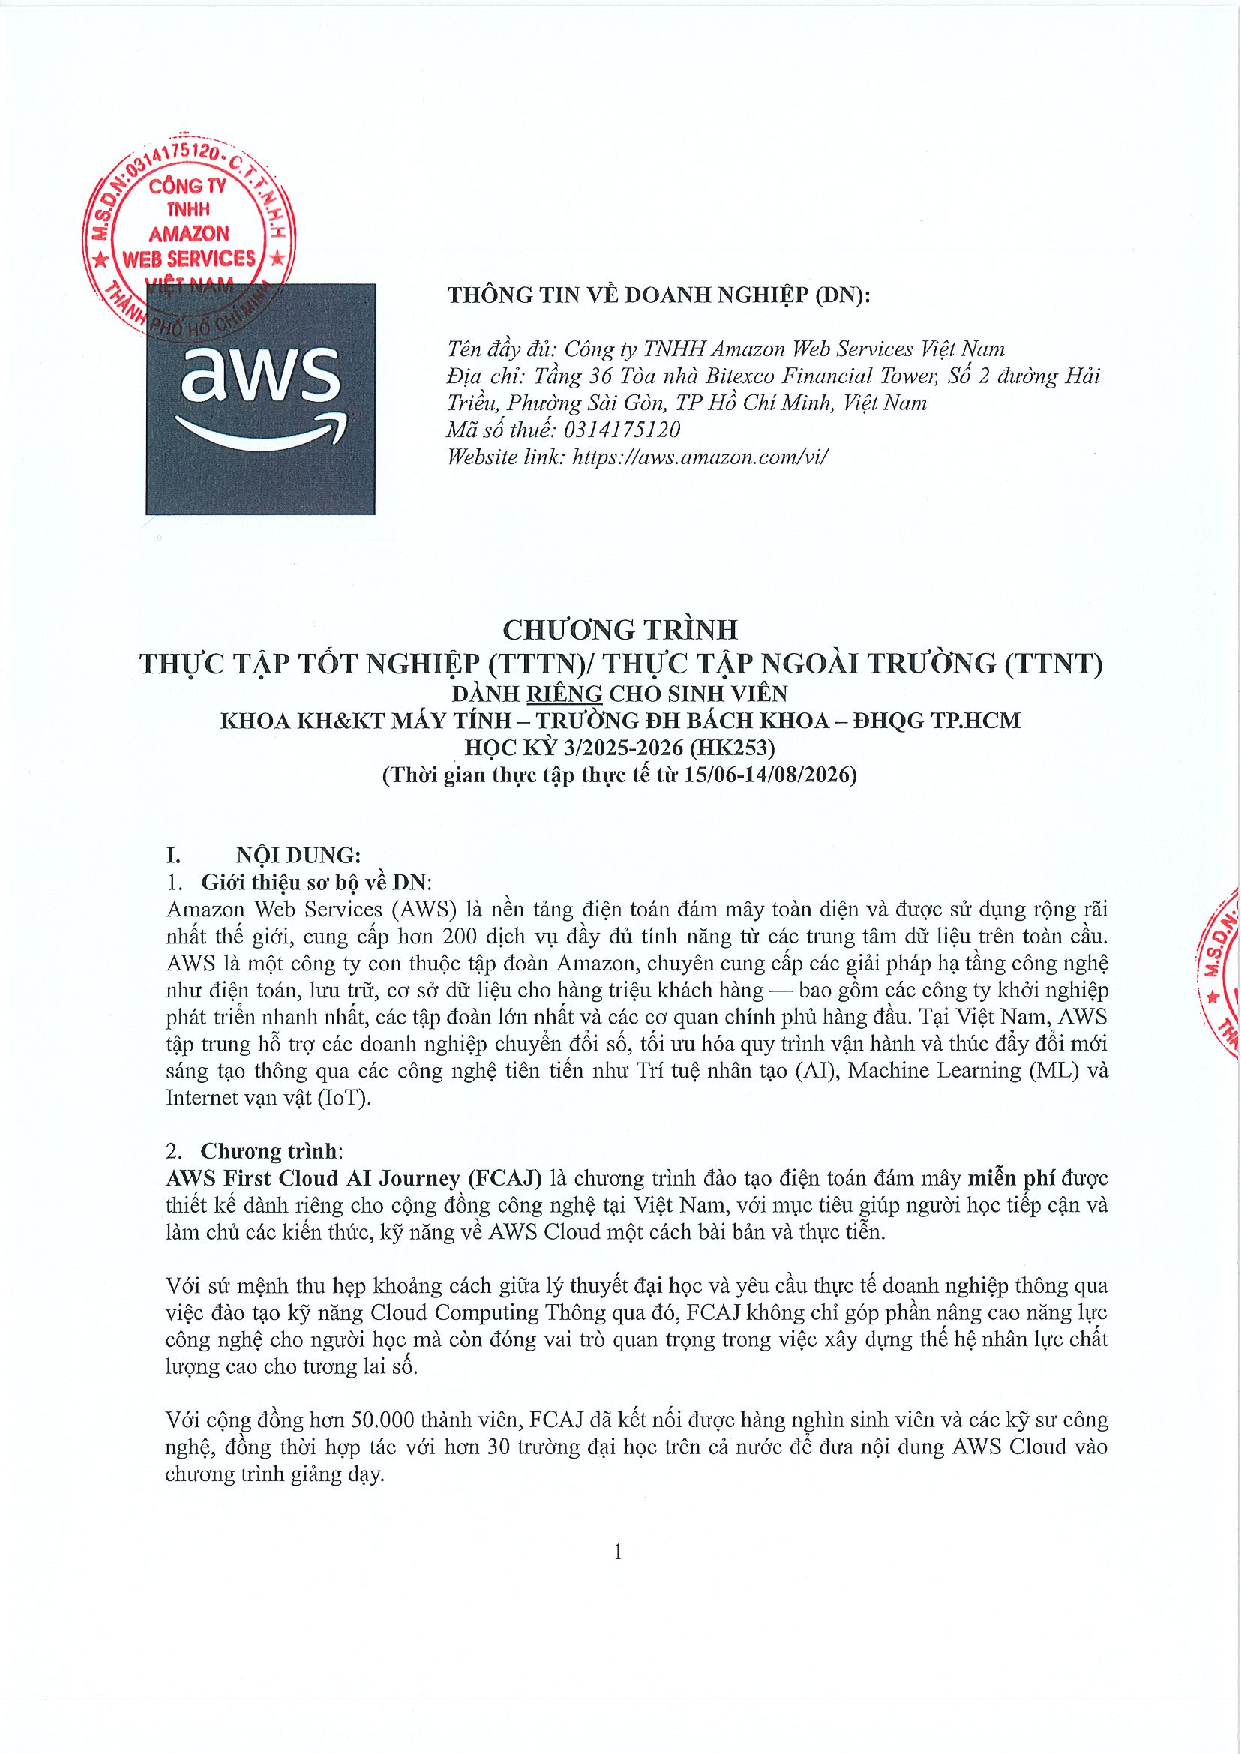
\includepdf[
    pages=-,
    addtotoc={1,section,1,Internship Program,sec:internship-program},
    pagecommand={\thispagestyle{empty}}
  ]{form/formD2.pdf}
}{
    \refstepcounter{section}
    \phantomsection
    \addcontentsline{toc}{section}{\protect\numberline{\thesection}Internship Program}
    \begin{center}
        \textit{Attach form D2 here}
    \end{center}
    \pagebreak
}

\endinput

% Form D3 is attached as-is. See ChuongTrinhThucTap_en.tex for why the heading
% is not typeset with \section.
% addtotoc steps the section counter and writes the number itself.
\IfFileExists{form/formD3.pdf}{
  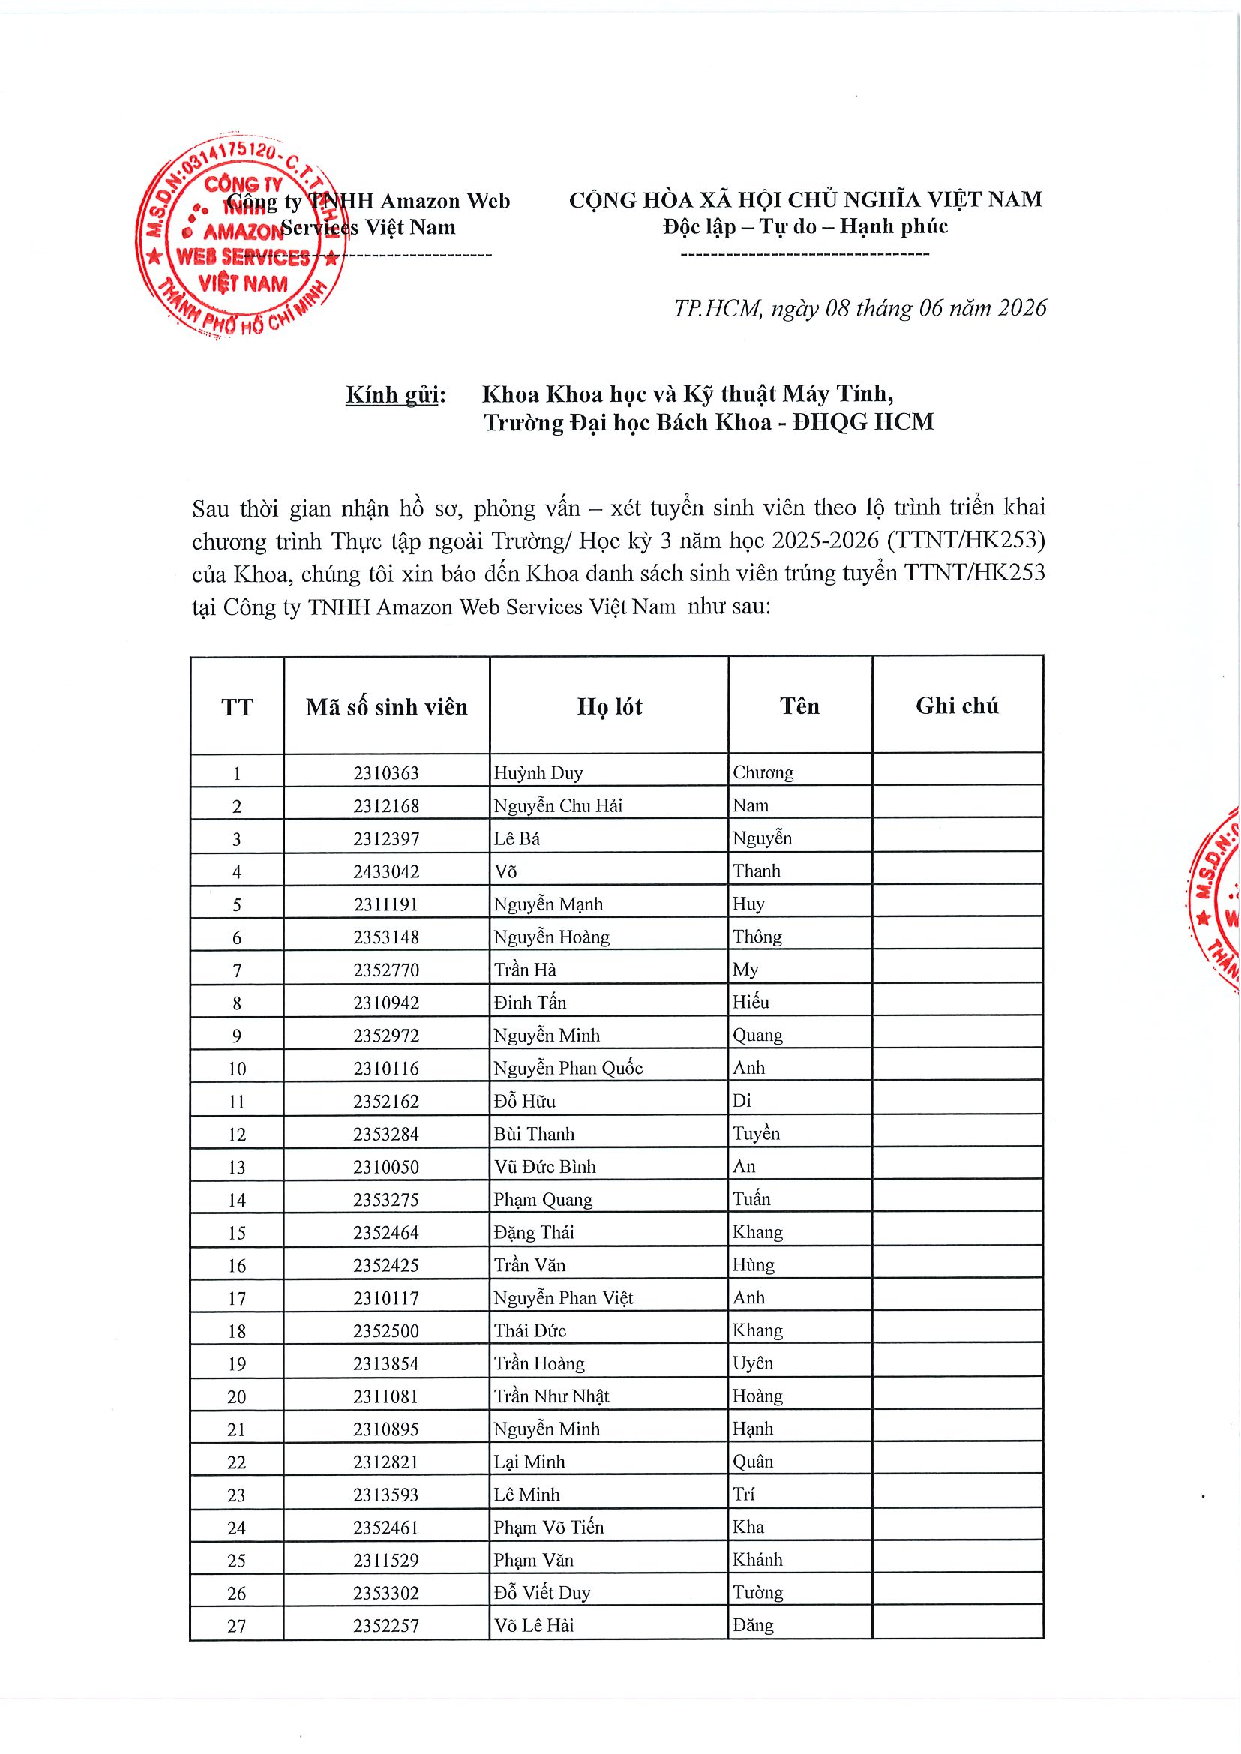
\includepdf[
    pages=-,
    addtotoc={1,section,1,Admission Results,sec:admission-results},
    pagecommand={\thispagestyle{empty}}
  ]{form/formD3.pdf}
}{
    \refstepcounter{section}
    \phantomsection
    \addcontentsline{toc}{section}{\protect\numberline{\thesection}Admission Results}
    \begin{center}
        \textit{Attach form D3 here}
    \end{center}
    \pagebreak
}

\endinput

\input{generated/content_body_en}

\newpage
\section{Summary}
\subsection{Skills and knowledge gained}

During my internship at \textbf{Amazon Web Services Viet Nam Company Limited},
from \textbf{15/06/2026} to \textbf{14/08/2026}, as part of the Workforce
Bootcamp -- First Cloud Journey programme, I moved from studying cloud computing
in theory to designing, building, and operating a complete system on AWS.

The first six weeks were spent working through the core service groups --
identity and access management, networking, compute, storage, databases,
serverless, and monitoring -- with a practical exercise attached to each. The
final weeks were spent applying all of it to \textbf{Caerus}, a cinema seat
booking platform built by a two-person team and deployed across Amazon EC2,
Amazon RDS, Amazon S3, API Gateway and Amazon CloudWatch.

The concrete skills I take away from the programme are:

\begin{itemize}
    \setlength\itemsep{0.2em}
    \item \textbf{Cloud architecture and service selection.} I can now design a
    multi-service architecture and justify each service choice against a
    specific alternative, rather than choosing by default.

    \item \textbf{Relational database design, transactional programming, and
    concurrency control.} Seat booking under concurrency turned out to be a
    transaction problem rather than a user-interface or infrastructure problem:
    lock the contested rows explicitly, acquire the locks in a consistent order
    to avoid deadlocks, and then prove the guarantee holds.

    \item \textbf{API design and working from a contract.} Agreeing the API
    specification and the database schema before writing any code is what
    allowed two people to build simultaneously instead of one waiting on the
    other.

    \item \textbf{Deployment and network security configuration}, including
    security groups, subnet placement, and the routing that connects them.

    \item \textbf{Observability and cost management.} Dashboards and alarms for
    the former; billing alarms, owner tags, and same-day teardown of practice
    resources for the latter.

    \item \textbf{Technical documentation.} Writing up architecture decisions
    and operating procedures so that someone who was not in the room can follow
    them.
\end{itemize}

In terms of work ethic, I kept to the schedule agreed at the start of the
project, maintained the daily habits the team committed to -- terminating
practice resources the same day and tagging every resource with its owner --
and raised problems with my teammate early rather than working around them
alone.

\subsection{What went well}

\begin{itemize}
    \setlength\itemsep{0.2em}
    \item \textbf{Learning breadth.} I began the programme with no practical AWS
    experience and finished it able to design a multi-service architecture and
    defend each service choice.

    \item \textbf{Working from a contract.} Freezing the API specification and
    the database schema up front was the single decision that kept the project
    on schedule. Integration became a matter of fixing small mismatches rather
    than reconciling two incompatible designs.

    \item \textbf{Solving the problem the project was actually about.} I
    verified the concurrency guarantee with a deliberate two-client race instead
    of assuming it held.

    \item \textbf{Cost discipline.} Setting a billing alarm before provisioning
    anything, tagging every resource with an owner, and terminating practice
    resources the same day meant cost never became a problem that had to be
    dealt with retrospectively.
\end{itemize}

\subsection{What I would do differently}

\begin{itemize}
    \setlength\itemsep{0.2em}
    \item \textbf{Proactiveness beyond the plan.} I executed the agreed schedule
    reliably, but tended to work through the task list rather than looking ahead
    and proposing improvements before they became necessary. Several issues we
    hit during deployment were foreseeable, and I should have raised them at
    design time instead of discovering them under time pressure.

    \item \textbf{Communication and presentation.} I am comfortable explaining
    technical decisions in writing, but less confident presenting them verbally
    to an audience that has not read the documents. This is the skill I would
    most like to develop next.

    \item \textbf{Depth beyond the working path.} Deployment is manual rather
    than automated, infrastructure was created through the console rather than
    defined as code, and automated testing is limited to the concurrency case
    rather than covering the API broadly.

    \item \textbf{Production-grade architecture.} The application runs on a
    single instance in a public subnet. I understand what a more robust
    deployment would involve -- private subnets with session-based access, a
    load balancer, an auto scaling group, and a multi-AZ database -- but I have
    not yet built one, so my knowledge of those patterns is conceptual rather
    than practical.

    \item \textbf{Estimating time.} My original estimates for deployment and
    cross-origin configuration were optimistic. The buffer days built into the
    plan absorbed the overrun, but the estimates themselves need to improve.
\end{itemize}

\subsection{Self-assessment}

To reflect objectively on the internship period, I evaluate myself against the
following criteria:

\begin{center}
\renewcommand{\arraystretch}{1.25}
\begin{tabular}{@{}c>{\raggedright\arraybackslash}p{7.2cm}ccc@{}}
\toprule
\textbf{No.} & \textbf{Criteria} & \textbf{Good} & \textbf{Fair} & \textbf{Average} \\
\midrule
1  & Professional knowledge \& skills & $\checkmark$ & $\square$ & $\square$ \\
2  & Ability to learn                 & $\checkmark$ & $\square$ & $\square$ \\
3  & Proactiveness                    & $\square$ & $\checkmark$ & $\square$ \\
4  & Sense of responsibility          & $\checkmark$ & $\square$ & $\square$ \\
5  & Discipline                       & $\checkmark$ & $\square$ & $\square$ \\
6  & Progressive mindset              & $\checkmark$ & $\square$ & $\square$ \\
7  & Communication                    & $\square$ & $\checkmark$ & $\square$ \\
8  & Teamwork                         & $\checkmark$ & $\square$ & $\square$ \\
9  & Professional conduct             & $\checkmark$ & $\square$ & $\square$ \\
10 & Problem-solving skills           & $\checkmark$ & $\square$ & $\square$ \\
11 & Contribution to project/team     & $\checkmark$ & $\square$ & $\square$ \\
12 & Overall                          & $\checkmark$ & $\square$ & $\square$ \\
\bottomrule
\end{tabular}
\end{center}

\subsection{Personal reflections}

The shape of the programme is what made the jump from theory to practice
possible. Six weeks of guided work through the core service groups, each with a
practical exercise, gave me enough ground to stand on that the final weeks could
be spent on a real system rather than on learning the console. Being asked to
build something end to end, and to justify the architecture rather than simply
assemble it, was far more instructive than any single service tutorial.

What I did not expect to value as much as I do is the operational discipline the
programme insisted on from day one: set the billing alarm before provisioning
anything, tag every resource with its owner, and terminate practice resources
the same day. Those habits cost almost nothing to maintain and removed an entire
category of problem from the project. They are the part of this internship I
expect to carry into every project afterwards.

Working in a pair taught me the rest. Agreeing an interface contract before
writing code is not process overhead; it is what let two people build in
parallel. I would like to thank my supervisor at the company and my faculty
supervisor for their guidance throughout the internship.

% The signatures get a page of their own, anchored at the top of it
% (\vspace* rather than \vspace, which would be dropped after a page break).
\newpage
\vspace*{1cm}

% Kept in one row so the two signatures never split across a page break.
\noindent
\begin{minipage}[t]{0.45\textwidth}
    \centering
    \textbf{Student}\\[0.2cm]
    % (Signature and full name)

    \vspace{2.2cm}

    \rule{0.8\linewidth}{0.4pt}
\end{minipage}
\hfill
\begin{minipage}[t]{0.45\textwidth}
    \centering
    \textbf{Company Representative}\\[0.2cm]
    % (Signature and full name)

    \vspace{2.2cm}

    \rule{0.8\linewidth}{0.4pt}
\end{minipage}

\end{document}
